\section{Centralized Authority}

A common way to implement auditability in private systems is to introduce a centralized authority or group of authorities (multi-party computation). Such authority can either be an external designated auditor or can enforce the internal policy rules in each transaction (accountability). 

According to this approach, users embed auxiliary information in the transactions, which is encrypted under the public key of a designated trusted auditor (\autoref{fig:cent-aud}). Thus, the users' data remains private to the rest of the system's participants, except for the central authority, which can decrypt the auxiliary information at any time without the users' consent. 

\begin{figure}
    \centering
    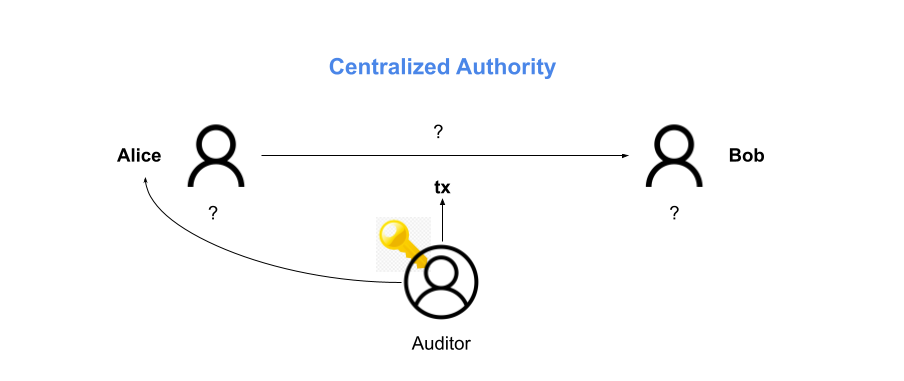
\includegraphics[width=0.9\textwidth]{images/privacy/Auditability in blockchain - Centralized.png}
    \caption{Auditability - Centralized Authority}
    \label{fig:cent-aud}
\end{figure}


This method can be a trivial solution for adding auditability to privacy-preserving systems. However, all data is collected by a single centralized authority, which accumulates excessive power. This fact can have a negative impact on user privacy.

An example that implements this approach is presented below:

\subsection{Zcash extension}
% \subsection{PRCash}
% \subsection{ACCDET}


\section{General Auditor}

To avoid collecting all information at a centralized authority (or group of authorities), a second approach has been proposed. This is an interactive protocol between the user being audited and the auditor. In this case, the auditor, which can be \textit{any} auditing authority, can ask specified questions derived from the system's policies. Users answer these questions with zero-knowledge proofs based on data stored on chain (\autoref{fig:gen-aud}).

This protocol implies the consent and cooperation of the audited user. However, this requirement cannot be exploited by non-compliant users, since refusal to cooperate with authorities can be considered equivalent to a failed audit.

\begin{figure}
    \centering
    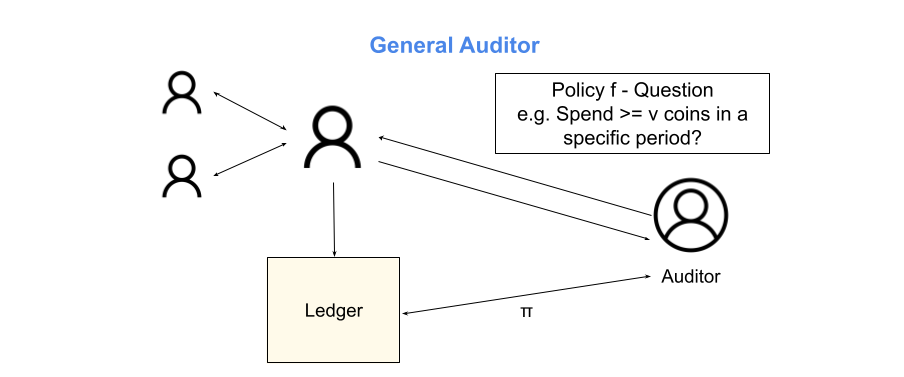
\includegraphics[width=0.9\textwidth]{images/privacy/Auditability in blockchain - General Auditor.png}
    \caption{Auditability - General Auditor}
    \label{fig:gen-aud}
\end{figure}

Below are some typical examples of auditable private decentralized systems that implement a general auditor:
\subsection{zkLedger}
% \subsection{miniLedger}
\subsection{PGC}